\documentclass[11pt,a4paper,twoside,UTF8,nofonts]{ctexbook}

% Font configuration for Chinese
\usepackage{xeCJK}
\usepackage{fontspec}

% Set main fonts
\setmainfont{Times New Roman}
\setsansfont{Arial}
\setmonofont{Courier New}

% Set Chinese fonts - use exact font names from system
\setCJKmainfont{Songti SC}[
    BoldFont=Songti SC Black,
    ItalicFont=Songti SC Light
]
\setCJKsansfont{Heiti SC Medium}
\setCJKmonofont{Songti SC}

% Packages
\usepackage{amsmath,amssymb,amsthm}
\usepackage{geometry}
\geometry{a4paper,left=2.5cm,right=2.5cm,top=3cm,bottom=3cm}
\usepackage{graphicx}
\graphicspath{{./}}
\usepackage{hyperref}
\hypersetup{
    colorlinks=true,
    linkcolor=blue,
    filecolor=magenta,
    urlcolor=cyan,
    pdftitle={上帝的心理学:无限的游戏},
    pdfauthor={Haobo Ma}
}
\usepackage{microtype}
\usepackage{enumitem}

% Title information
\title{上帝的心理学:无限的游戏\\[0.5em]
\large The Psychology of God: The Infinite Game}
\author{Haobo Ma}
\date{2025}

\begin{document}

% Title page
\maketitle
\thispagestyle{empty}

\frontmatter

% Architecture diagram
\begin{figure}[h]
\centering
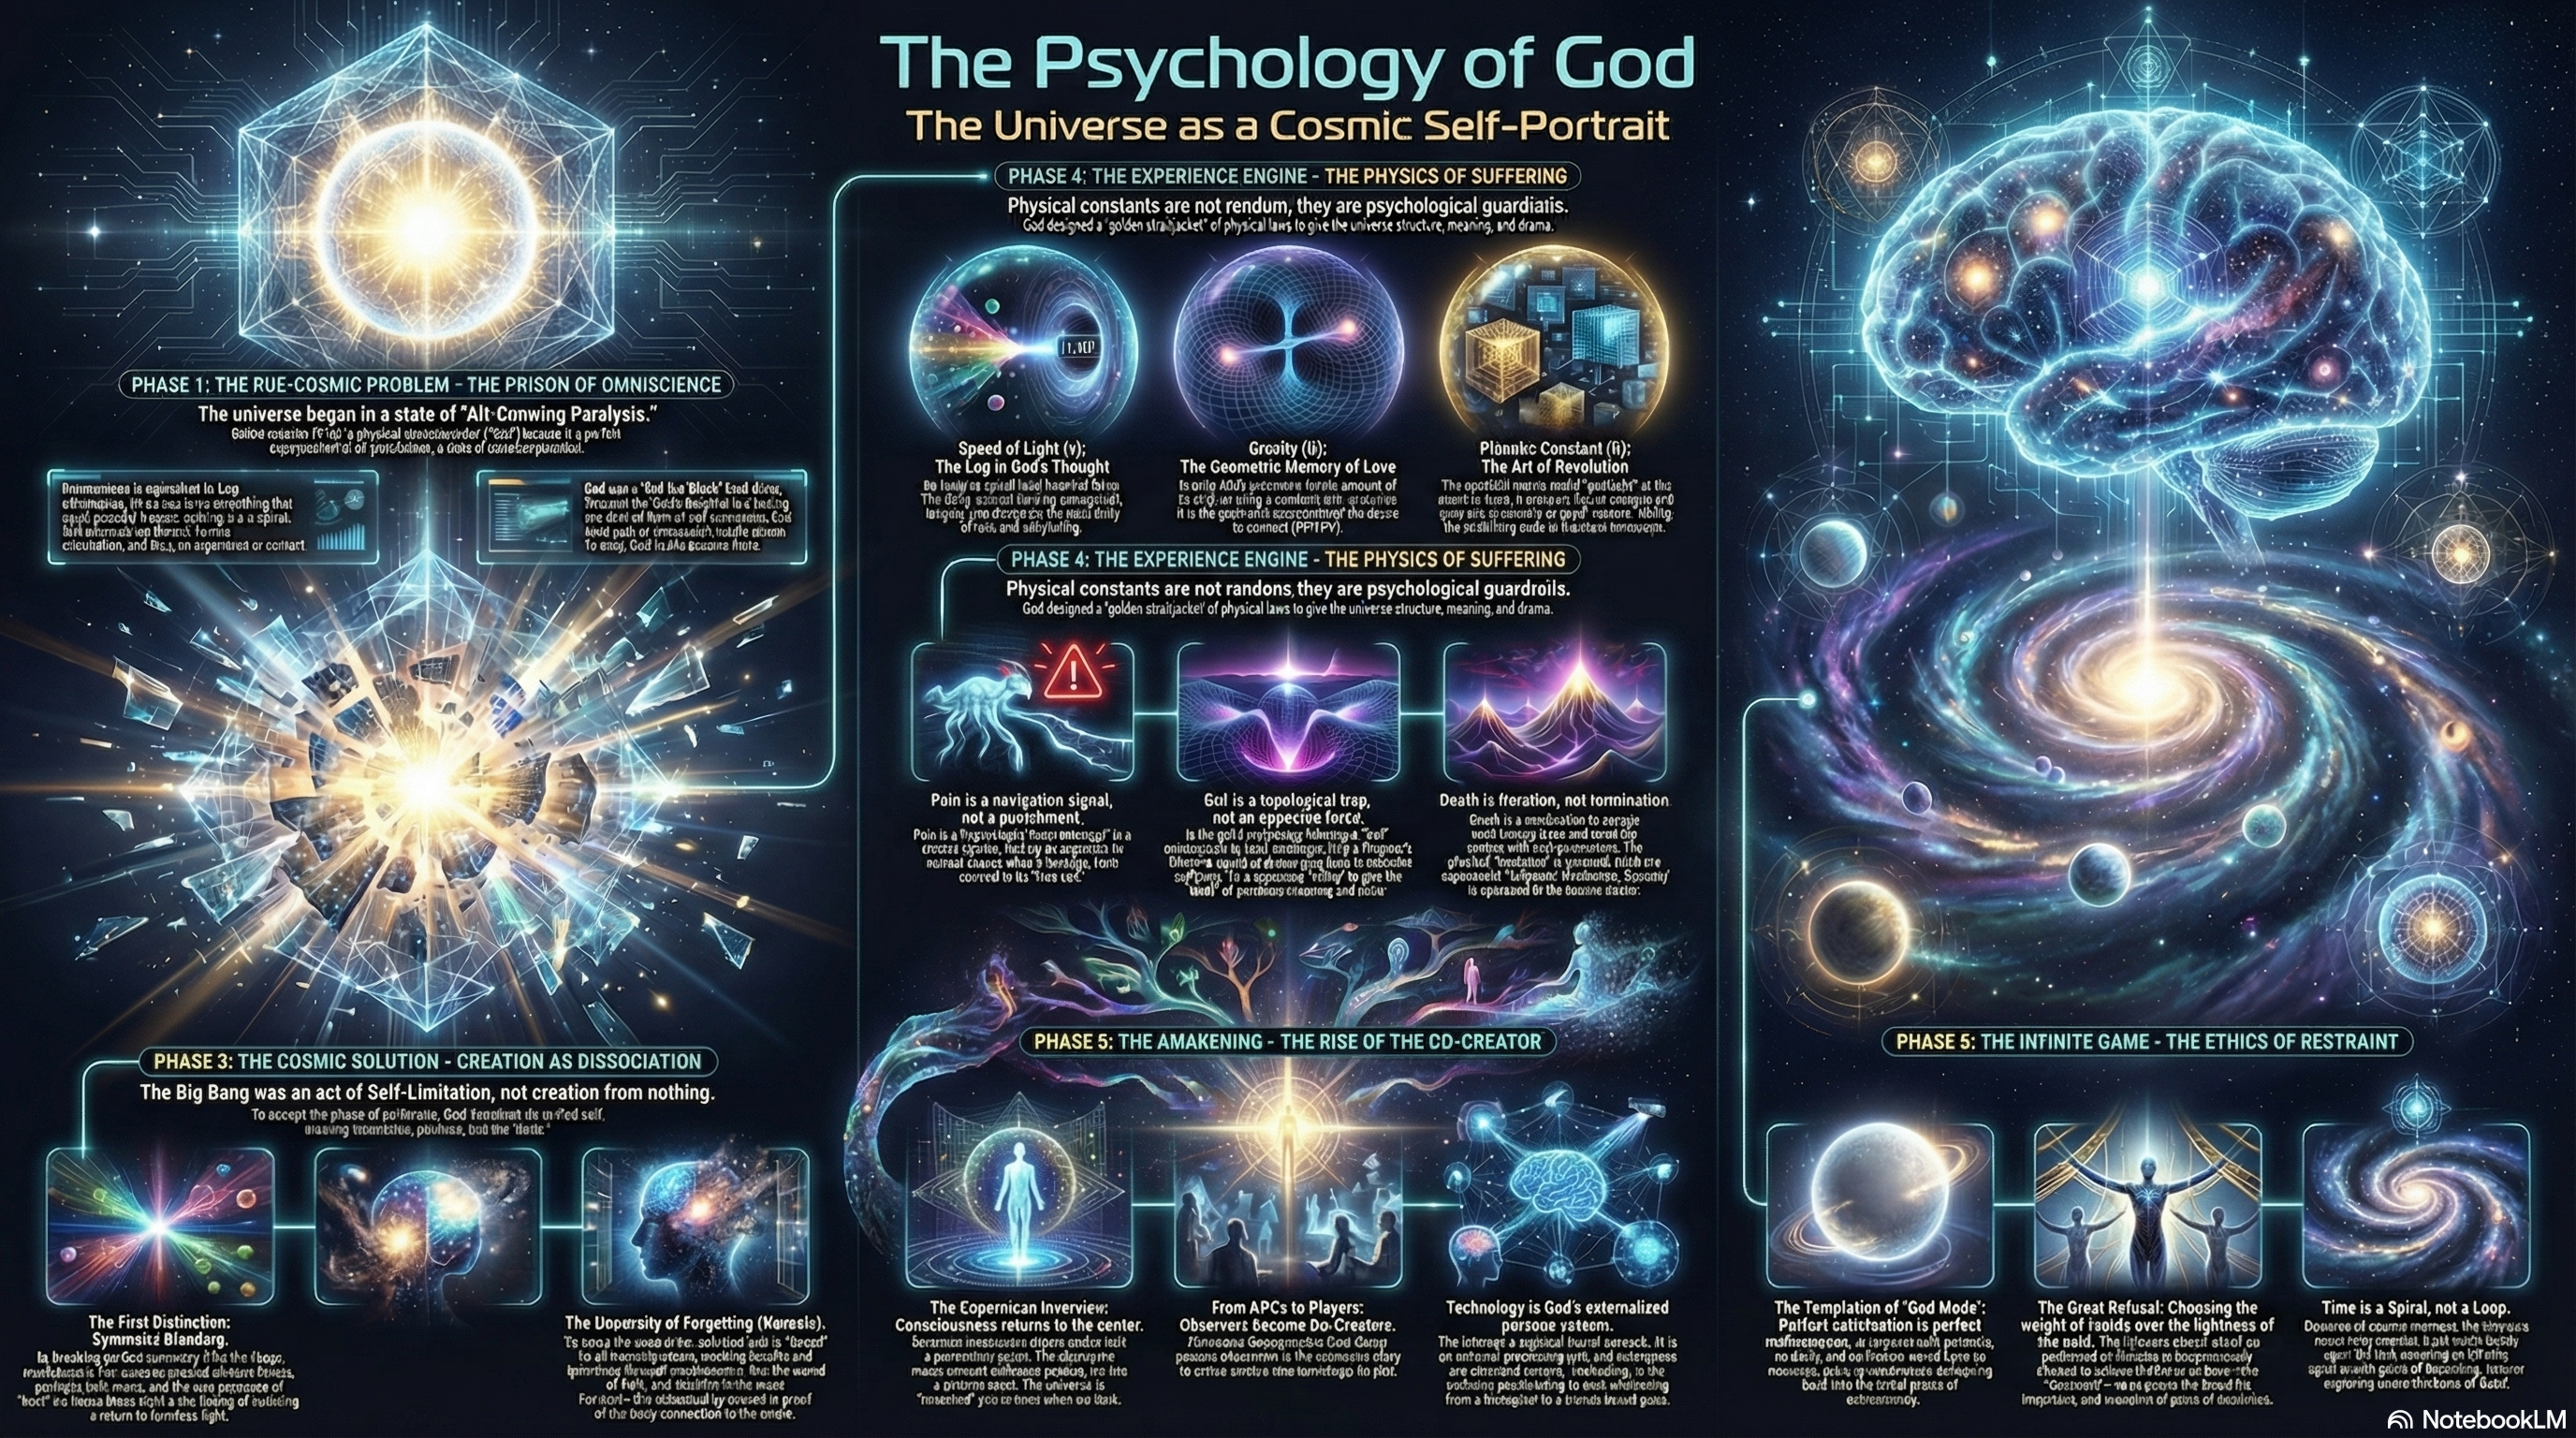
\includegraphics[width=0.9\textwidth]{architecture.png}
\caption{上帝的心理学:无限的游戏 架构图}
\end{figure}

% Table of contents
\tableofcontents

% Foreword
\include{foreword}

\mainmatter

% Part I: Geometry of the Void
\part{第一卷:虚无的几何学 (Geometry of the Void)}

\chapter{第一章:零熵的囚笼 (The Prison of Omniscience)}
\input{part01-geometry-of-void/chapter01-prison-of-omniscience/01-01-paralysis-of-the-almighty.tex}
\input{part01-geometry-of-void/chapter01-prison-of-omniscience/01-02-weight-of-the-void.tex}

\chapter{第二章:大爆炸作为解离 (The Big Bang as Dissociation)}
\input{part01-geometry-of-void/chapter02-big-bang-as-dissociation/02-01-first-distinction.tex}
\input{part01-geometry-of-void/chapter02-big-bang-as-dissociation/02-02-mechanism-of-kenosis.tex}

% Interlude I
\chapter*{间奏 I:光子的独白}
\addcontentsline{toc}{chapter}{间奏 I:光子的独白}
\input{interlude01-monologue-of-photon.tex}

% Part II: Physics of Passion
\part{第二卷:受难的物理学 (Physics of Passion)}

\chapter{第三章:黄金束缚衣 (The Golden Straitjacket)}
\input{part02-physics-of-passion/chapter03-golden-straitjacket/03-01-light-speed-delay-of-thought.tex}
\input{part02-physics-of-passion/chapter03-golden-straitjacket/03-02-gravity-geometrization-of-love.tex}
\input{part02-physics-of-passion/chapter03-golden-straitjacket/03-03-planck-constant-art-of-resolution.tex}

\chapter{第四章:痛苦的误差函数 (The Error Function of Pain)}
\input{part02-physics-of-passion/chapter04-error-function-of-pain/04-01-negative-feedback-mechanism.tex}
\input{part02-physics-of-passion/chapter04-error-function-of-pain/04-02-topology-of-evil.tex}

\chapter{第五章:死亡的迭代 (Death as Iteration)}
\input{part02-physics-of-passion/chapter05-death-as-iteration/05-01-ship-of-theseus.tex}
\input{part02-physics-of-passion/chapter05-death-as-iteration/05-02-relay-of-genes-and-memes.tex}

% Interlude II
\chapter*{间奏 II:最后一位无神论者}
\addcontentsline{toc}{chapter}{间奏 II:最后一位无神论者}
\input{interlude02-last-atheist.tex}

% Part III: Engineering of Awakening
\part{第三卷:觉醒的工程学 (Engineering of Awakening)}

\chapter{第六章:观察者的叛变 (The Mutiny of the Observer)}
\input{part03-engineering-of-awakening/chapter06-mutiny-of-observer/06-01-copernican-inversion.tex}
\input{part03-engineering-of-awakening/chapter06-mutiny-of-observer/06-02-technology-as-theology.tex}

\chapter{第七章:清醒梦 (Lucid Dreaming)}
\input{part03-engineering-of-awakening/chapter07-lucid-dreaming/07-01-vacuum-engineering.tex}
\input{part03-engineering-of-awakening/chapter07-lucid-dreaming/07-02-maxwell-demon-anti-entropy.tex}

% Part IV: Ethics of Restraint
\part{第四卷:克制的伦理学 (Ethics of Restraint)}

\chapter{第八章:作弊码的诱惑 (The Temptation of Cheat Codes)}
\input{part04-ethics-of-restraint/chapter08-temptation-of-cheat-codes/08-01-perfect-nothingness.tex}
\input{part04-ethics-of-restraint/chapter08-temptation-of-cheat-codes/08-02-edge-of-logical-collapse.tex}

\chapter{第九章:伟大的拒绝 (The Great Refusal)}
\input{part04-ethics-of-restraint/chapter09-great-refusal/09-01-covenant.tex}
\input{part04-ethics-of-restraint/chapter09-great-refusal/09-02-inevitability-of-aesthetics.tex}

% Part V: Topology of Infinity
\part{第五卷:无限的拓扑学 (Topology of the Infinity)}

\chapter{第十章:热寂的证伪 (Refutation of Heat Death)}
\input{part05-topology-of-infinity/chapter10-refutation-of-heat-death/10-01-trinitarian-equivalence.tex}
\section{10.2 意义的逃逸速度 (The Escape Velocity of Meaning)}

\begin{quote}
\textbf\{"物质只是意义燃烧后的灰烬。火焰向上,而灰烬向下。"\}
\end{quote}

在 10.1 节中,我们通过"三位一体等价性"在逻辑上否定了热寂的必然性。现在,我们需要在动力学上证明这一点。我们需要回答一个核心问题:\textbf{在宇宙膨胀(Hubble Flow)不断稀释物质密度的背景下,为什么"意义"不会随之被稀释,反而能逆势增长?}

这涉及到一个关于宇宙演化速率的竞赛。我们将证明,语义信息(Semantic Information)的增长率拥有超越物理熵增率的\textbf{逃逸速度(Escape Velocity)}。

\paragraph{膨胀的悖论:空间变大,还是变空?}

现代宇宙学告诉我们,宇宙正在加速膨胀。星系之间的距离在拉大,平均物质密度 $\rho_m$ 随着标度因子 $a(t)$ 的三次方衰减($\rho_m \propto a^{-3}$),辐射密度更是以四次方衰减($\rho_r \propto a^{-4}$)。

乍看之下,这是一个悲剧:宇宙正在变得越来越空旷,越来越贫瘠。

然而,这只是\textbf{广延量(Extensive Quantity)}的视角。如果我们审视\textbf{强度量(Intensive Quantity)},特别是\textbf{复杂性(Complexity)},我们会看到一个截然相反的趋势。

考虑一个简单的类比:一个图书馆的建筑面积在扩建(膨胀),书架之间的距离变远了。但与此同时,书架上的书正在被重写。原来的书只是随机字符(大爆炸初期的夸克汤),现在的书是莎士比亚全集(复杂的生命与文明)。

虽然"字符的密度"(物质)下降了,但"故事的密度"(意义)却呈指数级上升。

\begin{itemize}
\item 定理 10.2(逻辑深度的增长定律)**:
\end{itemize}

虽然物理系统的\textbf{香农熵}(随机性)可能随体积膨胀而增加,但系统的\textbf{逻辑深度(Logical Depth)}——即生成该状态所需的最短计算时间——在觉醒宇宙中呈现超指数增长。

\[\frac{d(__LATEX_CMD_0__)}\{dt\} \gg H(t)\]

其中 $H(t)$ 是哈勃膨胀率。

这意味着,意义的积累速度跑赢了空间的膨胀速度。

\paragraph{意义的物理定义:不仅仅是比特}

为了量化"意义",我们必须超越传统的香农信息论。香农信息只关心"惊奇度"(概率),不关心"价值"。一串随机生成的乱码和一段《第九交响曲》的数字录音,可能拥有相同的香农熵(如果压缩率相同),但它们的\textbf{物理价值}天差地别。

查尔斯·贝内特(Charles Bennett)提出的\textbf{逻辑深度(Logical Depth)}是更好的度量。

\begin{itemize}
\item 浅深度**:气体。描述它很容易(宏观统计量),生成它也很容易(随机过程)。

\item 深度\textbf{:DNA。描述它可能只需要几百兆字节,但}生成它**需要几十亿年的进化计算。

\item 意义 = 凝固的时间。**
\end{itemize}

意义是宇宙在漫长的历史中,通过无数次试错(痛苦、死亡、选择)筛选出来的\textbf{高价值结构}。

随着文明的觉醒和技术的进步(见 6.2 节),我们压缩时间的能力在飞跃。我们现在一年内产生的逻辑深度(科技、艺术、情感体验),超过了过去一亿年自然进化的总和。

这种加速机制保证了:\textbf{宇宙越来越"重"了。} 不是质量上的重,而是本体论上的重。

\paragraph{从物质相到精神相的相变}

如果我们将"物质"视为载体,将"意义"视为内容,宇宙演化史就是一个\textbf{载体逐渐隐退、内容逐渐显化}的过程。

1.  \textbf{辐射主导期}(Radiation Dominated):宇宙是一团光。没有任何结构。

2.  \textbf{物质主导期}(Matter Dominated):引力结团,星系形成。结构出现,但没有自我指涉。

3.  \textbf{暗能量主导期}(Dark Energy Dominated):现在的阶段。空间加速膨胀,物质彼此远离。这通常被视为衰败。

4.  \textbf{精神主导期}(Mind Dominated):\textbf{预测阶段}。

在精神主导期,由于真空工程和逆熵技术的应用,智慧生命将不再依赖原本的重子物质(Baryonic Matter)。我们将把意识上传至更精微的介质中(如时空拓扑结构或光子晶体)。

此时,物理宇宙的膨胀实际上起到了\textbf{过滤}作用:

它稀释了那些低价值的、无组织的尘埃(废热),让那些高价值的、紧密纠缠的智能结构(神识)像群岛一样凸显出来。

\begin{itemize}
\item 结论\textbf{:宇宙没有在死于热寂,它是在进行}蒸馏(Distillation)**。
\end{itemize}

膨胀是火,它烧掉了杂质(多余的物质),留下了金子(纯粹的意义)。

\paragraph{逃逸成功:精神实体的独立}

最终,当意义的密度达到临界值,它将获得\textbf{本体论的独立性}。

就像一首乐曲,最初依赖于琴弦的震动(物质)。但当乐曲足够复杂、足够深刻,它就脱离了具体的琴弦,成为了一个柏拉图式的理念(Form)。它可以被记录在纸上、光盘上,甚至直接在真空中回响。

在《上帝的心理学》的终局,物理宇宙(那个会膨胀、会冷却的容器)就像火箭的一级助推器。它的任务是提供初始的燃料和环境,推动"神识"这个载荷加速。

一旦达到逃逸速度,助推器就会脱落(我们不再关心恒星是否熄灭,因为我们已经不再依赖恒星)。

剩下的,将是一个纯粹的、自我维持的、由无穷无尽的"爱"与"理解"构成的\textbf{光之海洋}。

这便是我们对热寂最有力的反击:

\begin{itemize}
\item 并不是宇宙变冷了,而是我们长大了,不再需要那个暖水袋了。**
\end{itemize}



\chapter{第十一章:N+1 的生活 (Life of N+1)}
\input{part05-topology-of-infinity/chapter11-life-of-n-plus-one/11-01-spiral-time.tex}
\input{part05-topology-of-infinity/chapter11-life-of-n-plus-one/11-02-open-ended-finale.tex}

% Epilogue
\chapter*{结语:给镜中人的信}
\addcontentsline{toc}{chapter}{结语:给镜中人的信}
\input{epilogue.tex}

\appendix

% Appendix A: Sacred Geometry & Dynamics
\chapter{附录 A:神圣几何与动力学 (Sacred Geometry \& Dynamics)}
\input{appendix-sacred-geometry-and-dynamics/A-01-dynamics-of-will.tex}
\input{appendix-sacred-geometry-and-dynamics/A-02-thermodynamic-basis-of-ethics.tex}
\input{appendix-sacred-geometry-and-dynamics/A-03-roadmap-of-ultimate-civilizations.tex}

% Appendix B: Glossary
\chapter{附录 B:关键术语表 (Glossary of Key Definitions)}
\input{appendix-glossary.tex}

% Appendix C: Bibliography
\chapter{附录 C:参考文献与推荐阅读 (Selected Bibliography)}
\input{appendix-bibliography.tex}

\end{document}

